\subsection*{Courbes de Bézier}
\noindent
\subsubsection*{Paramétrisation}
\noindent
On nous donne $n+1$ points de contrôle $P_0, P_1, \dots,
    P_n$ et on veut définir une courbe de Bézier $B(t)$ qui passe par ces points.
\begin{equation}
    B(t) = \sum_{i=0}^{n} P_i\cdot B_i^n(t)=\sum_{i=0}^{n} P_i\cdot \binom{n}{i}\cdot t^i\cdot (1-t)^{n-i}
    \nonumber
\end{equation}
\subsubsection*{Algorithme de De Casteljau}
\noindent
On veut trouver les points de construction $b_0^1$, $b_1^1$, $b_0^2$ de la courbe de Bézier.
\begin{center}
    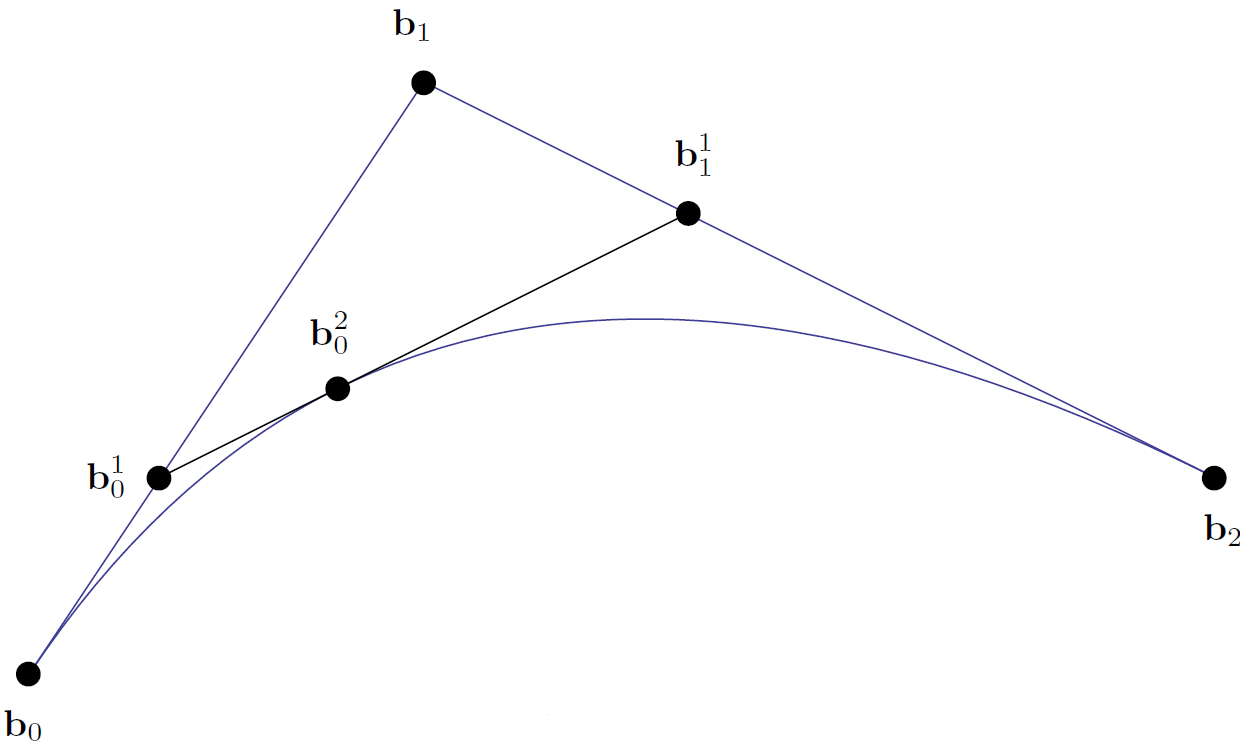
\includegraphics[width=0.275\textwidth]{images/bezier.png}
\end{center}
\begin{equation}
    \begin{tabular}{ccc}
        $b_0$ &         &         \\
        $b_1$ & $b_0^1$ &         \\
        $b_2$ & $b_1^1$ & $b_0^2$ \\
    \end{tabular}
    \nonumber
\end{equation}
Par exemple, pour les points $b_0=\binom{1}{1}, b_1=\binom{2}{\sfrac{5}{2}}, b_2=\binom{4}{\sfrac{3}{2}}$ et le pas $t=\sfrac{1}{3}$, on a:
\begin{equation}
    \begin{tabular}{ccc}
        $\begin{bmatrix}1 \\1\end{bmatrix}$            &                                                            &                                                              \\
        $\begin{bmatrix}2 \\\sfrac{5}{2}\end{bmatrix}$ & $\begin{bmatrix}\sfrac{4}{3} \\\sfrac{3}{2}\end{bmatrix}$  &                                                              \\
        $\begin{bmatrix}4 \\\sfrac{3}{2}\end{bmatrix}$ & $\begin{bmatrix}\sfrac{8}{3} \\\sfrac{13}{6}\end{bmatrix}$ & $\begin{bmatrix}\sfrac{16}{9} \\\sfrac{31}{18}\end{bmatrix}$ \\
    \end{tabular}
    \nonumber
\end{equation}
Ces points intermédiaires sont calculés comme suit:
\begin{equation}
    \begin{aligned}
         & b_0^1(t) = (1-t)\cdot b_0 + t\cdot b_1,     \\
         & b_1^1(t) = (1-t)\cdot b_1 + t\cdot b_2,     \\
         & b_0^2(t) = (1-t)\cdot b_0^1 + t\cdot b_1^1.
    \end{aligned}
    \nonumber
\end{equation}